%************************************************
\chapter{Antiferromagnetic resonance in a Rashba honeycomb antiferromagnet} % $\mathbb{ZNR}$\
%************************************************
\section{Introduction}
In the absence of spin-orbit interaction the spin of a conducting electron is conserved. In other words, its spin-life-time is infinite. In a conducting ferromagnet this means that collisions of electrons off of impurities cannot produce a finite spin-polarization and therefore any spin-orbit torque is absent. Furthermore, any rotation of magnetization leaves the electronic spectrum of the conducting electrons unchanged, as such a rotation is identical to a unitary transformation. Gilbert damping then, defined as the response of the spin of conducting electrons to the time-derivative of magnetization, must also be identically zero. Ferromagnets have therefore rather trivial and boring dynamics. In a conducting antiferromagnet however, this is not the case. Here independent rotations of magnetizations on both sublattices do not leave the spectrum invariant, but only a simultaneous rotation of both magnetizations in both sublattices leave the spectrum invariant, which means that the angle between the two magnetization directions must be a conserved quantity. With such a conservation intact, it has the important consequence that the spin on each sublattice is no longer conserved locally and we are allowed to move angular momentum from one sublattice to the other.   

In this Chapter we investigate the role of Rashba spin orbit interaction on the exchange Gilbert damping in a honeycomb antiferromagnet. We find that when the band splitting due to spin orbit is much smaller than the disorder-induced level broadening, disorder averaging will lead to a titanically large value of exchange Gilbert damping, which reflects the fact that it requires many scattering events to randomize the spin of a conducting electron. In the opposite limit where the spin-split bands can indeed be resolved the damping becomes suppressed by many orders of magnitude. Furthermore the damping becomes ultimately anisotropic which was the topic of the previous Chapter. We report that in the antiferromagnetic resonance spectrum we can directly see the effect of the exchange damping. In the large damping regime the magnetic system becomes overdamped and no resonance can be observed. The resonance appears to get a maximum value when the spin-orbit coupling has a value equal to the inverse momentum life-time of conducting electrons. 

Before introducing our model system, let us briefly make a few general observations about conducting antiferromagnets. Consider two magnetization vectors $\bb{m}_\text{A}$ and $\bb{m}_\text{B}$ on two sublattices of a antiferromagnet and furthermore conducting electrons with spin-polarizations $\bb{s}_\text{A(B)}$. An exchange interaction $\Delta$ couples the spin degree of freedom with the magnetization on each sublattice locally, leading to the following equations of motion on magnetization vectors
\beml
\label{basicEQ}
\begin{align}
\dot{\bb{n}}^\textrm{A}  & = \bb{H}^\textrm{A}\times\bb{n}^\textrm{A}  + (J\mathcal{A}/\hbar)\,\bb{n}^\textrm{A}\times \bb{s}^\textrm{A},\\
\dot{\bb{n}}^\textrm{B} & = \bb{H}^\textrm{B}\times\bb{n}^\textrm{B} +(J\mathcal{A}/\hbar)\,\bb{n}^\textrm{B}\times \bb{s}^\textrm{B},
\end{align}
\eml
where $\bb{H}$ is an effective field, $\mathcal{A}$ is the area of the unit cell, and $J$ and $\hbar$ are the (local) exchange energy and reduced Planck's constant ($h/2\pi$) respectively. 

We are interested in the response tensor $\alpha$ relating the spin-polarizations with the time-derivative of magnetizations
\begin{equation}
\label{eq:basicGilbert}
    \begin{pmatrix}
    \bb{s}_\text{A} \\ \bb{s}_\text{B}
    \end{pmatrix}
    =
    \begin{pmatrix}
    \alpha_{11}  &  \alpha_{12} \\ \alpha_{21}  &  \alpha_{22}
    \end{pmatrix}
    \begin{pmatrix}
    \partial_t \bb{m}_\text{A} \\ \partial_t\bb{m}_\text{B}
    \end{pmatrix}.
\end{equation}
The first observation we make is that the presence of sub-lattice-symmetry (the interchanging of the labels $A\leftrightarrow B$) necessarily leads to $\alpha_{11}=\alpha_{22}=\alpha_0$ and $\alpha_{11}=\alpha_{22}=\alpha'$. As written in the introduction when spin-orbit interaction is absent the angle between magnetizations $\bb{m}_\text{A}$ and $\bb{m}_\text{B}$ must be conserved. By inserting Eq.~(\ref{eq:basicGilbert}) into Eq.~(\ref{basicEQ}) we immediately find that $\alpha_0=\alpha'$ so that the damping tensor can be entirely described by the single number $\alpha_0$. Next we introduce the non-staggered and staggered magnetizations 
\begin{equation}
    \bb{m} = \bb{m}_\text{A} + \bb{m}_\text{B}, \quad \bb{n} = \bb{n}_\text{A} - \bb{n}_\text{B},
\end{equation}
and their equations of motion
\begin{align}
    \partial_t{\bb{n}}   & = \bb{H}\times\bb{n}  + \alpha_0 J\mathcal{A}/\hbar\,\bb{n}\times \partial_t\bb{m}\\
    \partial_t{\bb{m}}   & = \bb{H}\times\bb{m}  + \alpha_0 J\mathcal{A}/\hbar\,\bb{m}\times \partial_t\bb{m},
\end{align}
from which one can immediately see that the modulus of both $\bb{m}$ and $\bb{n}$ are conserved. Alternatively one can reach the same conclusion by noting that $\partial_t (\bb{m}_\text{A}\cdot\bb{m}_\text{B}) = \partial_t (m^2-n^2) = 0$ and that by construction $n^2+m^2=1$, from which it immediately follows that $\bb{m}\cdot\partial_t\bb{m} = \bb{n}\cdot\partial_t\bb{n} = 0$. 


\section{Role of vertex-corrections on the asymptotic behavior of $\alpha_{m,zz}$ and $\alpha_{m,\parallel}$}
It was shown in the previous Chapter that in the limit $\lambda\tau\ll1$ the damping tensor becomes isotropic, while in the opposing limit we find an ultimate anisotropy where $\alpha_{m,zz}$ vanishes completely. In the latter limit, the spin-split bands are completely resolved and certain spin-flip processes become forbidden. A more quantitative discussion on how $\alpha_{m,zz}$ and $\alpha_{m,\parallel}$ however, will be presented here. 

It is instructive to illustrate the role of disorder averaging in both limits as it turns out, the role of vertex-corrections on the components of the $\alpha_m$ tensor has a profound effect when $\lambda\tau/\hbar\ll1$, but negligible when $\lambda\tau/\hbar\gg1$. 

In the limit $\Delta_\text{sd}$ we are able to obtain concise and exact analytical formulas, that we present first. In this limit the exchange damping tensor can be fully characterized by just two numbers, $\alpha_m=\diag\left(\alpha_{m,\parallel}, \alpha_{m,\parallel}, \alpha_{m,zz}\right)$.

We will annotate the tensor-components with a superscript $(i)$, that denotes the number of disorder-lines inserted into the diagram. Physically, it means averaging over various disorder ensembles where the electron scatters $i$ number of times. 

Let us first consider the ``bare bubble'' contribution which describes an electron entering and exiting the system without a single scattering event
\begin{align}
    \alpha_{m,zz}^{(0)} =  & \frac{\varepsilon\tau}{\hbar} \frac{1-(\lambda/2\varepsilon)^2}{1+(\lambda\tau)^2},\\
    \alpha_{m,\parallel}^{(0)} =  & \frac{\varepsilon\tau}{\hbar}\left(\frac{1}{2}\frac{3+2(\lambda\tau/\hbar)^2}{1+(\lambda\tau/\hbar)^2}-\frac{2}{(4-\lambda/\varepsilon)^2}\right),
\end{align}
where one can immediately see the asymptotic behaviour for large and small values of $\lambda\tau$:
\begin{align}
    \alpha_{m,zz}^{(0)}  & = \frac{\epsilon\tau}{\hbar}\begin{cases}
    1  +\mathcal{O}(\lambda/\varepsilon)  & \text{ for }\lambda\tau/\hbar\ll1\\
    \hbar/(\lambda\tau)^2 & \text{ for }\lambda\tau/\hbar\gg1
    \end{cases},\\
    \alpha_{m,\parallel}^{(0)}  & = \frac{\epsilon\tau}{\hbar}\begin{cases}
    1  +\mathcal{O}(\lambda/\varepsilon)  & \text{ for }\lambda\tau/\hbar\ll1\\
    1/2 + \hbar/2(\lambda\tau)^2 & \text{ for }\lambda\tau/\hbar\gg1.
    \end{cases}
\end{align}
Evidently, the exchange damping transitions from fully isotropic to ultimately anisotropic when changing the limits $\lambda\tau\ll1$ to $\lambda\tau\gg1$. 
Including a small number of scattering events in the calculation we find an interesting modification:
\begin{align}
    \alpha_{m,zz}^{(i)}  & = \frac{\epsilon\tau}{\hbar}\begin{cases}
    i + \mathcal{O}(\lambda/\varepsilon)  & \text{ for }\lambda\tau/\hbar\ll1\\
    \hbar/(\lambda\tau)^2 & \text{ for }\lambda\tau/\hbar\gg1,
    \end{cases}\\
    \alpha_{m,\parallel}^{(i)}  &  = \frac{\epsilon\tau}{\hbar}\begin{cases}
    i + \mathcal{O}(\lambda/\varepsilon)  & \text{ for }\lambda\tau/\hbar\ll1\\
    1-(1/2)^{i+1}+\mathcal{O}(\hbar/(\lambda\tau)^2) & \text{ for }\lambda\tau/\hbar\gg1.
    \end{cases}
\end{align}
In the large $\lambda\tau$ limit the $zz$ component of the $\alpha_m$ tensor is unchanged by scattering events, whereas the parallel component quickly converges to the value of $\varepsilon\tau$. In the opposite limit, where the components remain isotropic with respect to each other, the components have a profound sensitivity to scattering events. Each scattering event contributes a value of $1\,\varepsilon\tau$ to the damping coefficient. While at a first glance it appears as strong sensitivity to impurities, it in reality reflects a long spin-life time: many scattering events are required to randomize the spin of an electron. 

In a truly diffusive system one should take the limit $i\rightarrow\infty$, in which case the tensor components are given by
\begin{align}
\label{eq:alphaparallelzerodelta}
    \alpha_{m,zz}^{(\infty)}  & = \frac{\epsilon \tau}{\hbar}\, \frac{2}{(2-n_z^2)\lambda^2\tau^2},\\
    \alpha_{m,\parallel}^{(\infty)}  & = \frac{\varepsilon\tau}{\hbar}\,\frac{2\,(1+\lambda^2\tau^2)}{(2-n_z^2)\lambda^2\tau^2}.
\end{align}

We plot the functions of $\alpha_{m,zz(\parallel)}^{(i)}$ for $i=0,1,2$ and $i\rightarrow\infty$ in Fig.~\ref{fig:alpha_plot}. 
\begin{figure}
    \centering
    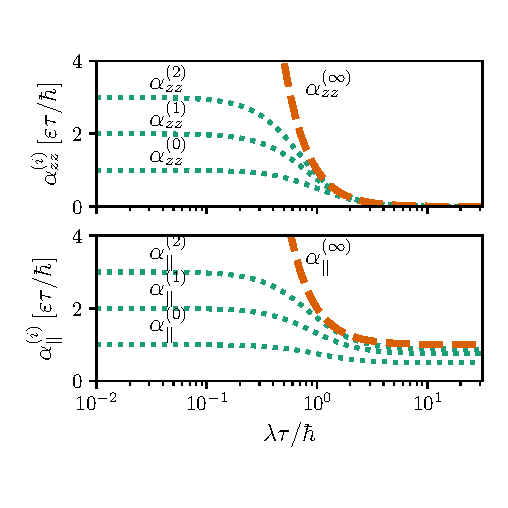
\includegraphics[width=\linewidth]{gfx/Chapter04/alpha_plot2}
    \caption{The first three scattering contributions $\alpha_{m,zz}^{(i)}$, $i=0,1,2$ (green, dotted) and the fully vertex corrected $\alpha_{m,zz}^{(\infty)}$ (orange, dashed) as a function of $\lambda \tau$. }
    \label{fig:alpha_plot}
\end{figure}
We find that indeed in the limit $\lambda\tau\gg1$ becomes ultimately anisotropic where $\alpha_{m,zz}$ becomes vanishly small. Moreover, we find a subtantial drop of $\alpha_{m,\parallel}$ for increasing values of $\lambda\tau$, that can reach a difference of many orders of magnitude. 

We note that a large value for damping corresponds to an overdamped regime, which we will explain in details in the next section. The direct exchange paramater $\Delta$ can be included perturbatively in both overdamped and underdamp regimes. In the overdamped regime,  $\Delta$ merely introduces a cutoff whereas in the underdamped regime a small modification.
\begin{align}
\label{eq:alphaparallelzerodelta}
    \alpha_{m,zz}^{(\infty)}  & = \frac{\epsilon \tau}{\hbar}\, \frac{2}{(2-n_z^2)\lambda^2\tau^2+2\Delta^2/\varepsilon^2},\\
    \alpha_{m,\parallel}^{(\infty)}  & = \frac{\varepsilon\tau}{\hbar}\,\frac{2(1+\lambda^2\tau^2)}{(2-n_z^2)\lambda^2\tau^2+2\Delta^2/\varepsilon^2}.
\end{align}
{\color{blue} Need to find correct coefficients for the underdamped regime ($\lambda\tau\gg1$)}
that we illustrate in Fig.~\ref{fig:alpha3}.
\begin{figure}
    \centering
    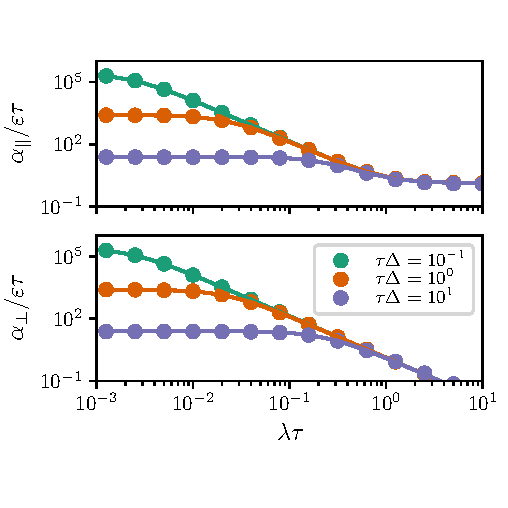
\includegraphics{gfx/Chapter04/alpha_plot1.pdf}
    \caption{Fully dressed damping components $\alpha_{\parallel,\perp}$ as a function of $\lambda\tau$ for three values of $\Delta\tau$. Note the use of log-scale on both horizontal and vertical axes.}
    \label{fig:alpha3}
\end{figure}
{\color{blue} (Need to check/update the coefficients and limits. }
%
% uniform modes
%
\section{Uniform modes in collinear ground state}
When subjecting an AFM to an oscillating magnetic field, the localized spins will exhibit a precession parallel to the magnetic field direction. By tuning the magnetic field's frequency to an internal harmonic frequency we can observe resonance. As shown first by Kittel and Keffer \cite{PhysRev.82.565, PhysRev.85.329} the resonance frequency is proportional to the square root of the product of anisotropy and exchange energy. The width of the resonance frequency however, as we show below, is linearly proportional to anisotropy and exchange damping. Although exchange damping remains finite, even large, at vanishingly small values of spin-orbit interaction, the anisotropy must vanish. A direct calculation from the grand potential (see Appendix~\ref{app:D}), we find that the Rashba honeycomb lattice exhibits an out-of-plane and easy-axis anisotropy. Close to $\bb{n}=\bb{n}_\perp$ the magnetostatic anisotropy energy is given by
\begin{equation}
    E = -\frac{K}{2}n_z^2, \quad K= \frac{1}{2\pi\hbar^2v^2}\begin{cases}
    |\Delta^2\lambda|  &  \text{for } |\lambda/2\Delta| \geq 1 \\
    |\Delta\lambda^2|  &  \text{for } |\lambda/2\Delta| \leq 1
    \end{cases}.
\end{equation}

The transition from $|\lambda/2\Delta|\le1$ to $|\lambda/2\Delta|\ge1$ correspond to the merger of two of the bands as illustrated in Fig.~\ref{fig:bands}. The resonance frequencies and widths are obtained by including the effect of anisotropy in the equations of motion on $\bb{n}$ and $\bb{m}$
\beml
\label{AFMEOM2}
\begin{align}
\label{ndot2}
\dot{\bb{n}} = &  -\Omega\, \bb{n}\!\times\!\bb{m} +K \bb{m}\!\times\!\bb{n}_\perp+\bar{\alpha}_m\,\bb{n}\!\times\!\dot{\bb{m}}+\alpha_n\,\bb{m}\!\times\! \dot{\bb{n}},\\
\label{mdot2}
\dot{\bb{m}} = & K  \bb{n}\!\times\!\bb{n}_\perp+\alpha_n\,\bb{n} \times \dot{\bb{n}}+\bar{\alpha}_m \bb{m} \times \dot{\bb{m}} ,
\end{align}
\eml
To obtain the resonance frequency and width we follow a standard recipe of linearization \cite{kittel}. First expand the (non)-staggered magnetizations around the classical ground-state solution
\begin{align}
    \bb{n}\rightarrow\hat{\bb{z}} + \delta\bb{n}_\parallel,\quad \bb{m}\rightarrow \delta\bb{m}_\para,
\end{align} 
(where $\delta m_\perp$ is omitted to ensure that $\bb{n}\cdot\bb{m}=1+\mathcal{O}(\delta^2)$) and keep only first order contributions in the equations of motion of Eqs.~(\ref{AFMEOM2}). The harmonics $\omega$ are obtained by replacing $\partial_t \rightarrow i\omega$ through which we arrive at a linear system of equations. We find the real and imaginary parts of $\omega = \omega_0 + i \delta\omega$ to be
\begin{align}
    \omega_0 = \sqrt{K(\Omega + K(1- \alpha_m^2 / 4))},\quad \delta\omega =  \frac{K \alpha_m + \Omega \alpha_n }{2(1- \alpha_n \alpha_m)},
\end{align}
{\color{blue} or further to:
\begin{align}
    \omega_0 = \sqrt{K\Omega},\quad \delta\omega =  \frac{K \alpha_m}{2},
\end{align}
}
where we used that $\alpha_n\ll\alpha_m$.
% \be
% \omega = \frac{\sqrt{2 K(K+ \Omega)(1+ \alpha_m^\parallel \alpha_n - \alpha_n^2) + 4 K^2 - K^2 (\alpha_m^{\parallel})^2}}{2 +2 \alpha_n^2 - 2 \alpha_n \alpha_m^\parallel}
% \e
% Using that $\alpha_n\ll\alpha_m$,  we arrive at the more compact expression
% \be
% \re \omega = \sqrt{K(\Omega + K - K \alpha_m^2 / 4)}
% \e
% the width of the resonance line will be given by the imaginary part of the $\omega$:
% \be
% \delta\omega \equiv \im \omega = \frac{K (\alpha_m - 2 \alpha_n) + \Omega \alpha_n }{2 +2 \alpha_n^2 - 2 \alpha_n \alpha_m}.
% \e
The ratio $\delta\omega/\omega_0$ {\color{blue} does this have a name?} can be minimized with respect to $\lambda$ when $\lambda\tau\sim1$. In the limit $\Delta/\varepsilon\rightarrow0$ it can be seen from Eq.~(\ref{eq:alphaparallelzerodelta}) that the minimum is achieved at exactly $\lambda\tau=1$. For small values of $\Delta/\varepsilon$ the minimum is slightly shifted according to:
\begin{equation}
    \lambda\tau = 1 + \frac{8\Delta^2/\varepsilon^2}{2-n_z^2}+\mathcal{O}\Big(\frac{\Delta^4}{\varepsilon^4}\Big).
\end{equation}
In this limit we find after dropping $\alpha_n$ and neglecting terms $\mathcal{O}(K/\Omega)$ we get the result

% The in-plane damping that appears in the resonance frequency width can be minimized with respect to $\tau$ when $\lambda\tau/\hbar = 1$, which corresponds to \begin{equation}\alpha_{m,||}^{(\infty)}=\frac{\varepsilon}{\lambda}\frac{3-(\lambda/\varepsilon)^2}{1-(\lambda/2\varepsilon)^2}, \end{equation}
% the normalized resonance width  $\delta\omega/\omega$ is then given by
\begin{align}
    \frac{\delta\omega}{\omega}  & \simeq \frac{\sqrt{K}\alpha_m}{2\sqrt{\Omega}}\nonumber\\
     & \simeq\frac{1}{2\sqrt{2\pi}\hbar v}\frac{3\varepsilon}{\sqrt{\Omega}} \begin{cases}
    |\Delta/\sqrt{\lambda}|  &  \text{for } |\lambda/2\Delta| \geq 1 \\
    \sqrt{|\Delta|}  &  \text{for } |\lambda/2\Delta| \leq 1.
    \end{cases}
    \label{eq:freq}
\end{align}
We consider the regimes (1) The limit $\lambda\tau\ll1$ and $\Delta\ll\lambda$, (2) the limit $\lambda\tau\ll1$ and $\Delta\gg\lambda$, (3) $\lambda\tau=1$ and (4) $\lambda\tau\gg1$. For each regime we find:
\begin{align}
    (1) & \quad \frac{\delta\omega}{\omega}= \frac{1}{2\sqrt{2\pi} v}\frac{1}{\sqrt{\Omega}}\frac{\varepsilon\Delta}{\lambda^{3/2}\tau}\\
    (2) & \quad \frac{\delta\omega}{\omega}= \frac{1}{2\sqrt{2\pi} v\hbar^2}\frac{1}{\sqrt{\Omega}}\frac{\varepsilon^3\lambda\tau}{\Delta^{3/2}}\\
    (3) & \quad \frac{\delta\omega}{\omega}= \frac{1}{2\sqrt{2\pi}\hbar v}\frac{3\varepsilon}{\sqrt{\Omega}} \begin{cases}
    |\Delta/\sqrt{\lambda}|  &  \text{for } |\lambda/2\Delta| \geq 1 \\
    \sqrt{|\Delta|}  &  \text{for } |\lambda/2\Delta| \leq 1.
    \end{cases}\\
    (4) & \quad \frac{\delta\omega}{\omega}= \frac{\varepsilon\tau}{2\sqrt{2\pi} v\hbar^2}\frac{1}{\sqrt{\Omega}}
    \begin{cases}
    |\Delta\sqrt{\lambda}|  &  \text{for } |\lambda/2\Delta| \geq 1 \\
    |\sqrt{\Delta}\lambda|  &  \text{for } |\lambda/2\Delta| \leq 1.
    \end{cases} 
\end{align}
{\color{blue} Still have to edit above equations}

The ratio $\delta\omega/\omega$ is plotted for few values of $\Delta$ in Fig.~\ref{fig:freqs}
\begin{figure}
    \centering
    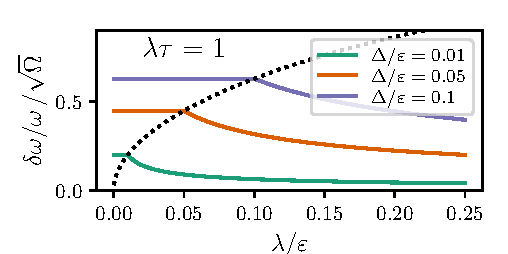
\includegraphics{gfx/Chapter04/freq_plot.pdf}
    \caption{Frequency for the optimal case $\lambda\tau=1$ for few values of $\Delta$. The black dotted curve corresponds to Eq.~(\ref{eq:freq}) for $\lambda=\Delta$}. 
    \label{fig:freqs}
\end{figure}